% !TEX root = main.tex
%\myparagraph{Key points}
%\begin{enumerate}[1.]
%%	\item	Session $\pi$ calculus with process passing. DONE
%%	\item	Identify session $\pi$ and process passing subcalculi and their polyadic variants. DONE
%%	\item	Bisimulation theory for higher-order session semantics. DONE
%%	\item	New triggered bisimulation, related to J\&R's. DONE
%%	\item   Elementary values key to characterizations of behavioural equivalence. DONE
%	\item	Types provide techniques to prove completeness without matching. \jp{TBD}
%	\item	We are interested in encodings with properties a la Gorla. 
%                We extended them to typed setting. \jp{TBD}
%%	\item	Encode name-passing to pure process abstraction calculus, with name abstractions. DONE
%%	\item	Type of the recursion encoding uses non tail recursive type $\trec{t}{\btinp{t} \tinact}$. DONE
%%	\item	Encode higher-order semantics to first order semantics. DONE
%%	\item	Negative result. Cannot encode shared names using only shared names.
%%	\item   Extensions with higher-order abstractions and polyadicity also explored. DONE
%\end{enumerate}

%\smallskip 
%
%\myparagraph{Important things to explain}
%Explain our \HO is very small without containg name passing 
%\[ 
%\abs{x}.P \quad \appl{x}{u}
%\]

%Explain we input only characteristic processes.  
%
%\[
%\lambda x.\mapchar{S}{x}
%\]

%\subsection{Higher-Order Session Calculi}
\noi 
This paper is about \emph{relative expressiveness} results for 
\emph{higher-order process calculi}, core programming languages that 
integrate name- and process-passing in communications.
We focus on higher-order languages coupled with \emph{session types} that denote interaction protocols. 
%The expressivity relations that we aim to are essential for the transference of reasoning techniques, notably behavioral equivalences, across different typed languages. 
%Our motivation for studying expressivity relations is to establish a firm foundation for the transference of reasoning techniques, notably behavioral equivalences, across different session typed languages. 
Results of relative expressiveness 
enable us to identify \emph{essential} process constructs that cannot be expressed in terms of other constructs. They are also central 
ingredients in the   \emph{transference of reasoning techniques}, notably behavioral theories, across different languages.
Since session types denote protocols, 
 establishing expressiveness results formally entails defining 
 not only a translation (\emph{encoding})
relating source and target languages, but also a translation 
relating their associated type systems. 
We thus aim at a very particular class of correct encodings: namely \emph{fully abstract} and \emph{type-preserving} encodings.
%This is a challenging task, as we elaborate next.
Next, we discuss further our goals and the challenges involved.

In \emph{session-based concurrency}, concurrent interactions are organized into \emph{sessions}, basic communication units.
Interaction patterns can then be abstracted as expressive \emph{session types}~\cite{honda.vasconcelos.kubo:language-primitives}, against which process specifications may be checked. 
These patterns are defined as %(possibly recursive) 
sequences of communication actions: % (send/receive a value, offer/select a behavior).
%For instance, 
%session type $T_1 = \btinp{\mathsf{str}} \btout{\mathsf{int}}  \tinact$ may be intuitively read as: receive (?) a value of type $\mathsf{str}$,then output (!) a value of type $\mathsf{int}$, finally close the protocol.
type $\btinp{U} S$ (resp.  $\btout{U} S$)
describes a protocol that first receives (resp. sends) a value of type $U$ and then continues as protocol $S$.
Also, given an index set $I$, types $\btbra{l_i:S_i}_{i \in I}$ 
and $\btsel{l_i:S_i}_{i \in I}$ 
define %, respectively,
%a branching and selection constructs for  
 a labeled choice mechanism; types 
$\trec{t}{S}$ 
and 
$\tinact$ denote recursive and completed protocols, respectively.
%describes a protocol that offers
%(resp. ) 
%Type $\tinact$ denotes the completed protocol.
In the (first-order) $\pi$-calculus~\cite{MilnerR:calmp1}, 
session types describe the intended interactive behavior of the names/channels in a process.
%names/channels are endowed with session types (such as $T_1$) representing their intended interactive behavior.
Session-based concurrency has also been casted in the setting of \emph{higher-order} process
calculi which, by combining features from the $\lambda$-calculus and the $\pi$-calculus, 
enable the exchange of values that may contain processes~\cite{tlca07,DBLP:journals/jfp/GayV10}. 
Besides offering a natural bridge between concurrent and functional computation, 
higher-order calculi with sessions enable the specification of structured protocols involving \emph{code mobility}, 
frequent in practice.
In the main higher-order session language that we study here (denoted \HOp),
 values in communications include names but also (first-order) abstractions---functions from name identifiers to processes. 
 %(In contrast, higher-order abstractions---functions from processes to processes---are disallowed.)
 (In contrast, functions from processes to processes are disallowed.)
Abstractions can be linear or shared; their value types are  denoted $\lhot{C}$ and $\shot{C}$, respectively ($C$ 
%is a first-order type $C$ (say, a session name).
denotes a name). We may then have 
session types such as
%$T_2 = \btbra{upload:\btinp{\lhot{\mathsf{int}}}\tinact ~ , ~ sha:\btinp{\shot{\mathsf{int}}}\tinact}_{}$
$$\btbra{up:\btinp{\lhot{C}}\btout{\mathsf{ok}}\tinact ~ , ~ down:\btout{\shot{C}}\btout{\mathsf{ok}}\tinact ~ , ~quit:\btout{\mathsf{bye}}\tinact}_{}$$
which abstracts the protocol of a server that allows 
  clients to select among distinct  behaviors: %namely, 
  to \emph{upload} a linear function (which the server is ready to receive), to \emph{download} a shared function (which the server is ready to send), or to \emph{quit} the protocol.
  In each case, the server sends a confirmation message ($\mathsf{ok}$ or $\mathsf{bye}$) before closing the session.




%The study of higher-order concurrency has received significant attention, 
%from untyped and typed perspectives (see, e.g.,~\cite{ThomsenB:plachoasgcfhop,SangiorgiD:expmpa,San96int,MostrousY15,DBLP:journals/iandc/LanesePSS11,DBLP:conf/icalp/LanesePSS10,DBLP:conf/esop/KoutavasH11,XuActa2012}),
%in particular via comparisons with the (first-order) $\pi$-calculus~\cite{MilnerR:calmp1}. 
%Higher-order calculi with {session primitives}, put forward in~\cite{tlca07,DBLP:journals/jfp/GayV10},
%allow for the specification of structured, reciprocal exchanges (protocols) 
%which can be verified via type-checking using {session types}~\cite{honda.vasconcelos.kubo:language-primitives}.
%Although models of session-typed 
%communication with features of higher-order concurrency exist
%their \emph{relative expressiveness}
%remains little understood. 
Roughly speaking, 
  \HOp %, a higher-order process language that 
extends Sangiorgi's higher-order $\pi$-calculus~\cite{SangiorgiD:expmpa} with session primitives.
More precisely, \HOp
includes
constructs for 
%session establishment
synchronisation along shared names, 
session communication (value passing and labelled choice) along linear names,
recursion, 
 (first-order) abstractions %(i.e., functions from name identifiers  to processes)
 and applications.
% (denoted $\lambda x.P$ and $(\lambda x.P)a$, resp.).
%While synchronization on shared names (useful to model session establishment) is 
%non deterministic, session communication is deterministic and occurs on linear names.
\HOp is therefore a rather rich process language. This immediately begs the question:
is there a \emph{sub-calculus} of \HOp with equal expressivity? %hich is as expressive as the whole calculus? 
In addition to its intrinsic foundational interest, this question also has practical ramifications, 
as such a \emph{core calculus} could be taken as reference in 
implementations of languages with session primitives.
In this way, expressiveness results may help in justifying connections 
between theoretical and more
practical advances in the design of (functional) programming languages with session types support.

%We have recently developed a behavioral theory  for \HOp~\cite{characteristic_bis}:
%we introduced
%\emph{characteristic bisimilarity}, a sound and complete 
%characterization of contextual equivalence. % that enables tractable analyses.


Previous studies already suggest two main sources 
of expressiveness in \HOp: \emph{name passing} and constructs for \emph{infinite behavior} (i.e., recursion and replication). 
For instance, name-passing calculi (both untyped and typed) are able to express the $\lambda$-calculus and 
process-passing calculi~\cite{SangiorgiD:expmpa}. In the $\pi$-calculus, recursion and replication can be expressed in terms of each other. 
In higher-order calculi,
these operators are redundant: they can be represented exploiting process duplication. 
Also, even higher-order calculi which lack name passing, restriction, and recursion are known to be quite expressive.
%For these reasons, 
Consequently, 
in this paper we study the expressivity of \HOp in relation to two  sub-calculi
that distill the essence of higher- and first-order session-based concurrency:
\begin{enumerate}[-]
\item the \HO-calculus: \HOp without recursion and name passing;
\item the session \sessp-calculus \jpc{(denoted~\sessp)}: \HOp without abstractions and applications.  
\end{enumerate}
%Interestingly, %\HO and \sessp distil the essence of higher- and first-order session-based concurrency:
While \sessp is, 
in essence, the first-order calculus in~\cite{honda.vasconcelos.kubo:language-primitives}, 
%this paper shows 
our main discovery is 
that \HO  is a new core calculus 
for higher-order session concurrency.
We assess the expressivity 
 of \HOp, \HO, and \sessp as delineated by session typing. 
We establish strong correspondences between 
these calculi  via type-preserving, fully abstract encodings up to 
behavioural equalities. 
%While encoding \HOp 
%into the $\pi$-calculus preserving session types 
%(extending  known  results for untyped processes~\cite{SangiorgiD:expmpa}) is 
%%\jpc{already}
%significant, 
Our main contribution is 
an encoding of \HOp into \HO (\secref{subsec:HOpi_to_HO}).  
Since \HO lacks 
both name-passing and recursion, this encoding involves two key challenges:
\begin{enumerate}[a.]
\item Known (typed) encodings of name-passing into process-passing~\cite[Ch.13]{SaWabook} are limited: % in that 
%they come with restrictions on name usages;  
they work for %name-passing 
calculi 
%with \emph{capability types} 
in which only the output capability of names is sent---a received name cannot be used in subsequent inputs.
This is far too limiting in \HOp, where 
 names denoting arbitrary protocols may be passed around (\emph{delegation})
and types describe  communication  \emph{structures}, rather than individual name capabilities. % at a given time.

\item In untyped higher-order calculi, 
forms of infinite behavior 
(such as recursion) % and replication)
can be encoded using process duplication. 
Unfortunately, this encoding does not carry over to session typed calculi such as \HOp,
because linear abstractions cannot be copied. Hence, the discipline of session types severely limits 
the possibilities for representing infinite behaviors---even simple forms, such as input-guarded replication.
\end{enumerate}




%MOTIVATION FIRST ENCODING (). \emph{Still to highlight: recursive type required, no recursion, small example.

%--- 
\noi
We describe our approach to these challenges.
Concerning (a), %we illustrate the essence of 
to encode name passing into \HO, 
%to encode name output, 
we ``pack''
the name to be passed around into a suitable abstraction; 
upon reception, the receiver must ``unpack'' this object following a precise protocol.
More precisely, our encoding 
\jpc{of name passing}
in \HO is given as:
\begin{center}
\begin{tabular}{rcll}
  $\map{\bout{a}{b} P}$	&$=$&	$\bout{a}{ \abs{z}{\,\binp{z}{x} (\appl{x}{b})} } \map{P}$ \\
  $\map{\binp{a}{x} Q}$	&$=$&	$\binp{a}{y} \newsp{s}{\appl{y}{s} \Par \bout{\dual{s}}{\abs{x}{\map{Q}}} \inact}$
\end{tabular}
\end{center}
%and as a homomorphism for the other operators.
%Above, 
where
$a,b$ are names and $s$ and $\dual{s}$ are 
linear session names (\emph{endpoints}).
%$\lambda x.P$ is a name abstraction of $P$; $\appl{x}{a}$ is a name application; 
Processes $\bout{a}{V} P$ and 
$\binp{a}{x} P$ denote output and input at~$a$;   
abstractions and applications are denoted
$\lambda x.P$ and $(\lambda x.P)a$, respectively;
$\newsp{s}P$ and $\inact$ represent hiding and the inactive process, respectively.
Thus, following a higher-order communication on $a$, %our encoding features 
a (deterministic) reduction between  
$s$ and $\dual{s}$ which guarantees that name $b$ is properly unpacked.

We stress that aiming at type-preserving encodings 
makes our endeavor more challenging, since it rules out encoding strategies that, while plausible, do 
not preserve session types. For instance, consider the 
encoding of %$\sessp$ 
name-passing 
into $\HO$ defined as
\begin{center}
\begin{tabular}{rcll}
  $\umap{\bout{a}{b} P}$	&$=$&	$\binp{a}{x}( \appl{x}{b} \Par \umap{P})$ \\
  $\umap{\binp{a}{x} Q}$	&$=$&	$\bout{a}{\abs{x}{\umap{Q}}} \inact$
\end{tabular}
\end{center}
and as a homomorphism for the other operators.\footnote{This alternative  encoding was suggested by an anonymous reviewed of a previous version of this paper.}
Intuitively, this encoding inverts communication prefixes: outputs are translated into inputs, and inputs are translated into outputs. 
As such, it is a perfectly reasonable encoding in an \emph{untyped setting}. However, the encoding $\umap{\cdot}$  is far from desirable in a session typed setting: since 
individual communication prefixes represent actions in a structured sequence of communications (as expressed and disciplined by session types)
the encoding $\umap{\cdot}$ would simply destroy the intrinsic meaning of session protocols in the source language.

Concerning (b),Encoding a recursive process $\recp{X}{P}$ is \NY{also} challenging, for 
the linearity of endpoints in $P$ must be preserved.
We encode recursion with non-tail recursive session types; for this 
we apply recent advances on the theory of session duality~\cite{TGC14,DBLP:journals/corr/abs-1202-2086}.
TO EXPAND.
%\dk{Encoding of a general recursive process $\recp{X}{P}$ is another challenge, since 
%it must preserve the linearity of session endpoints appeared in $P$.
%We encode it with non-tail recursive session types,  
%for which we apply a recent advance on a session duality theory 
%\cite{BernardiH14,TGC14,DBLP:journals/corr/abs-1202-2086}.}


TO ADD: MOTIVATION ON PRECISE AND MINIMAL ENCODINGS. We should also mention the non encodability result (\secref{ss:negative}).
(We should also mention the less surprising encoding in \secref{subsec:HOp_to_sessp}.) 
While encoding \HOp 
into the $\pi$-calculus preserving session types 
(extending  known  results for untyped processes~\cite{SangiorgiD:expmpa}) is 
%\jpc{already}
significant, 


MOTIVATION: EXTENSIONS (\secref{sec:extension}) -- We further extend our encodability results to 
i)~\HOp with \emph{higher-order} abstractions (denoted \HOpp) 
and to ii)~\HOp with polyadic name passing and abstraction (\pHOp); and to
their super-calculus  (\PHOpp) (equivalent to the calculus in~\cite{tlca07}). 
%Here again the usage information given by session types is essential to define encodings
%and to state their semantic correspondences.
% Building upon established notions for (untyped) processes~(e.g.,~\cite{DBLP:journals/iandc/Gorla10}), 
% we
%define a notion of \emph{precise encoding} that 
%requires the translation of both process and types, and 
%focuses on process mappings that preserve (session) typing. 
%Thus, our encodings only relate source and target 
%processes 
%with  
%proper communication structures (given by session types).
A further result shows that 
shared names
%as required in the session establishment phase,
strictly add expressive power 
to session calculi. 
\figref{fig:express} summarises %our expressivity 
these results. %including the three extensions of \HOp. 

\begin{figure}[t]
\centering
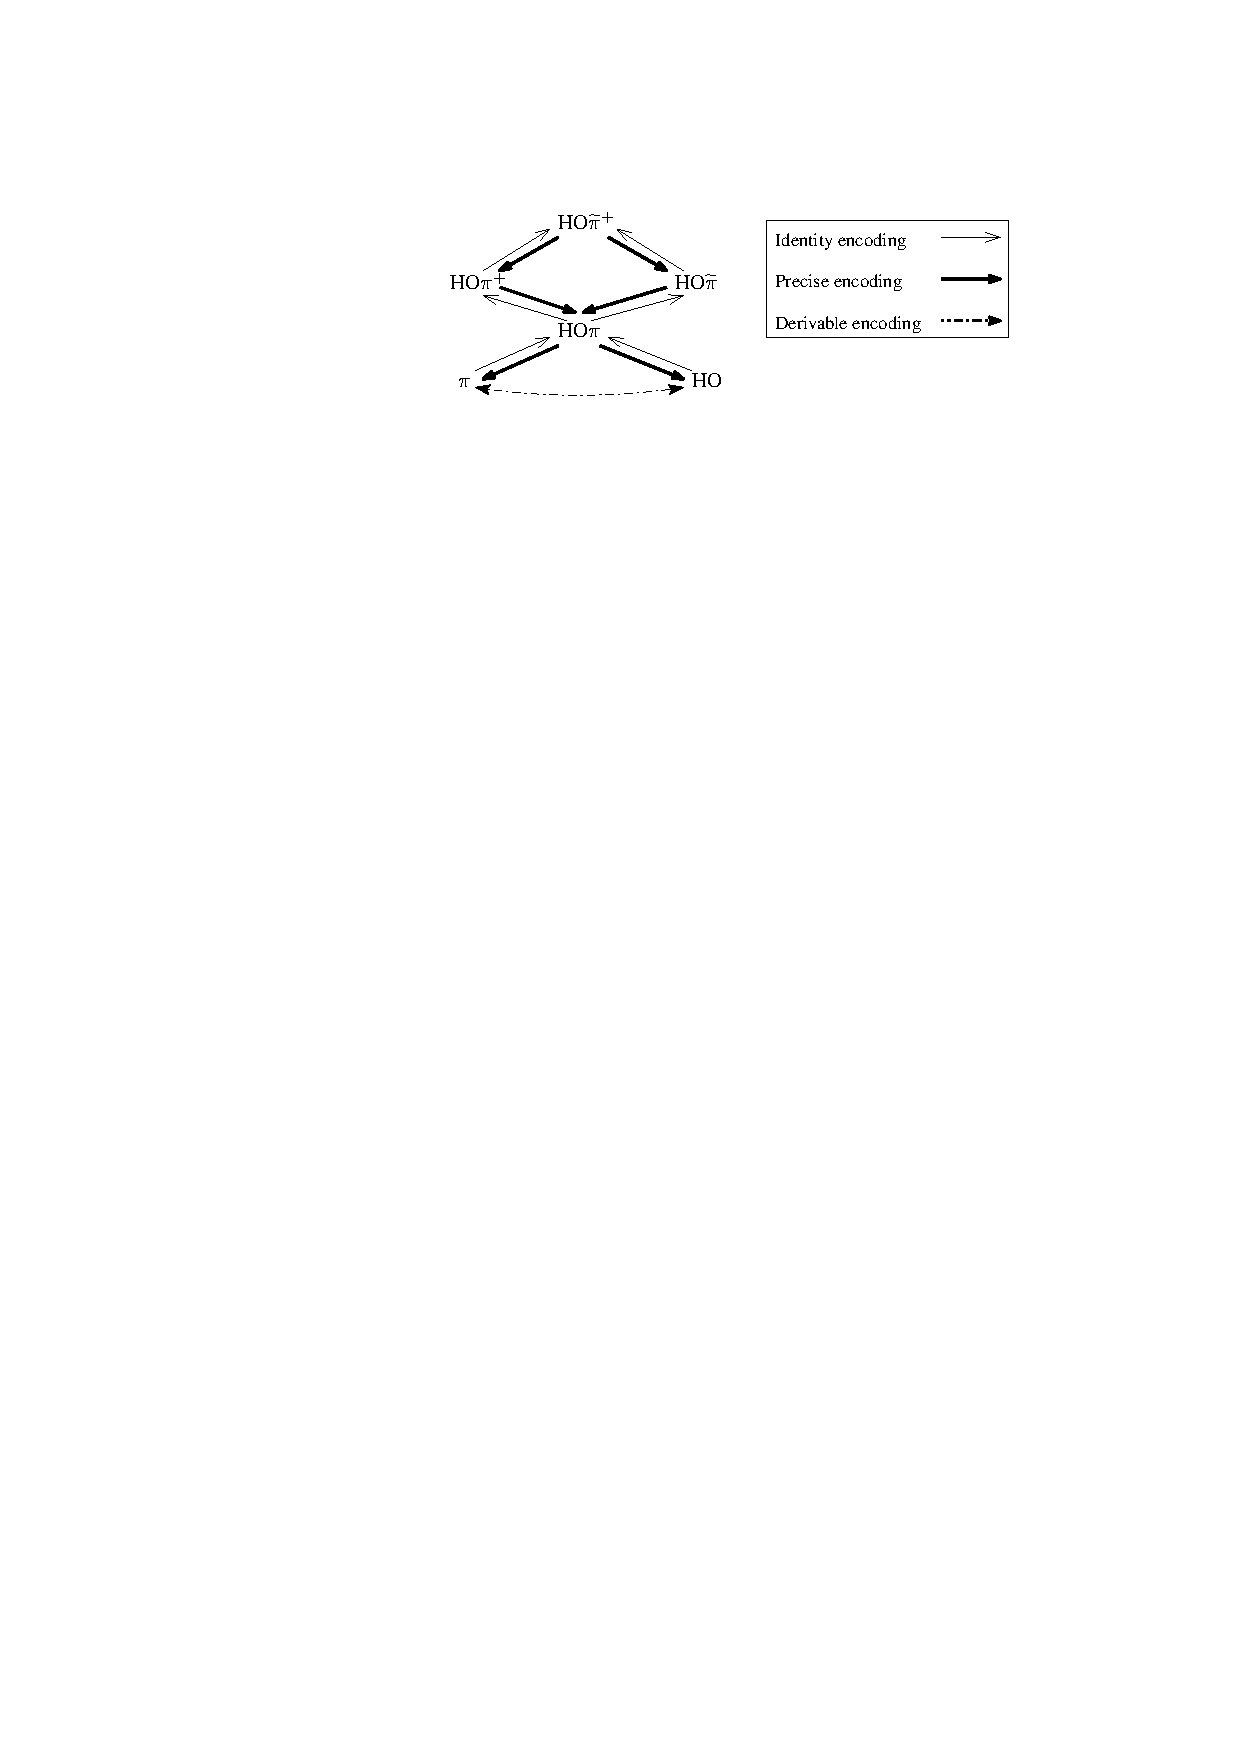
\includegraphics[scale=1]{diag.pdf}
\vspace{1mm}
%%ADD~FIGURE!
%	\centering
%	\begin{subfigure}[b]{0.45\linewidth}
%		\centering
%		\begin{tikzpicture}
%
%			\node	(PHOpp)	at	(0, 0.8)		{\PHOpp};
%			\node	(HOpp)	at	(-1.5, 0.4)	{\HOpp};
%			\node	(PHOp)	at	(1.5, 0.4)	{\PHOp};
%			\node	(HOp)	at	(0, 0)		{$\mathsf{HO}{\pi}^{~}$};
%			\node	(HO)	at	(-1.5, -0.4)	{$\mathsf{HO}{~}^{~}$};
%			\node	(sessp)	at	(1.5, -0.4)	{$~~\pi^{~}$};
%
%			\draw[<-]	(PHOpp) -- (HOpp);	%(0, 1.25) -- (-2, 1);
%			\draw[<-]	(PHOpp) -- (PHOp);	%(0, 1.25) -- (2, 1);
%
%			\draw[<-]	(HOpp) -- (HOp);	%(2, 0.5) -- (0, 0.25);
%			\draw[<-]	(PHOp) -- (HOp);	%(-2, 0.5) -- (0, 0.25);
%
%			\draw[<-]	(HOp) -- (HO);		%(0, -0.25) -- (-2, -0.5);
%			\draw[<-]	(HOp) -- (sessp);	%(0, -0.25) -- (2, -0.5);
%
%%				\node	(PHOpp)	at	(0, 0.8)		{\PHOpp};
%%				\node	(HOpp)	at	(-2, 0.4)	{\HOpp};
%%				\node	(PHOp)	at	(2, 0.4)	{\PHOp};
%%				\node	(HOp)	at	(0, 0)		{$\mathsf{HO}{\pi}^{~}$};
%%				\node	(HO)	at	(-2, -0.4)	{$\mathsf{HO}{~}^{~}$};
%%				\node	(sessp)	at	(2, -0.4)	{$~~\pi^{~}$};
%%
%%				\draw[->]	(PHOpp) -- (HOpp);	%(0, 1.25) -- (-2, 1);
%%				\draw[->]	(PHOpp) -- (PHOp);	%(0, 1.25) -- (2, 1);
%%
%%				\draw[->]	(HOpp) -- (HOp);	%(2, 0.5) -- (0, 0.25);
%%				\draw[->]	(PHOp) -- (HOp);	%(-2, 0.5) -- (0, 0.25);
%%
%%				\draw[->]	(HOp) -- (HO);		%(0, -0.25) -- (-2, -0.5);
%%				\draw[->]	(HOp) -- (sessp);	%(0, -0.25) -- (2, -0.5);
%		\end{tikzpicture}
%	\end{subfigure}
%%	\hfill
%	\begin{subfigure}[b]{0.5\linewidth}
%		\small
%		The arrow start calculus wrt arrow tip calculus:
%		\begin{itemize}
%			\item	is a sub-calculus.
%			\item	encodes.
%		\end{itemize}
%		Arrow properties are transitive.
%	\end{subfigure}
%\\
	\caption{Encodability in Higher-Order Sessions. 
	Precise encodings are defined in \defref{def:goodenc}.
	\label{fig:express}}
\Hlinefig
\end{figure}

\smallskip

\myparagraph{Outline / Contributions.} This paper 
is structured as follows:
\begin{enumerate}[$\bullet$]
\item \secref{sec:overview} overviews key ideas of our tractable bisimulations.
\item \secref{sec:calculus} presents the higher-order session calculus \HOp and its 
subcalculi \HO and \sessp.  Then, \secref{sec:types} gives the session type system
and states type soundness for \HOp and its variants.
%\item \secref{sec:behavioural} 
%develops \emph{higher-order} and \emph{characteristic} bisimilarities, our two
%tractable characterisations of contextual equivalence which 
%alleviate the issues of context bisimilarity~\cite{San96H}. These 
%relations are shown to coincide in \HOp (\thmref{the:coincidence}).
\item \secref{s:expr} defines \emph{precise (typed) encodings} by extending encodability criteria 
studied for
untyped processes~(e.g.~\cite{DBLP:journals/iandc/Gorla10,DBLP:conf/icalp/LanesePSS10}).
\item \secref{sec:positive} %and \S\,\ref{sec:negative}
gives encodings of \HOp into \HO and of \HOp into~\sessp.
These encodings 
are shown to be \emph{precise} (Thms.~\ref{f:enc:hopitoho} and~\ref{f:enc:hotopi}).
Mutual encodings between \sessp and \HO are derivable; 
all these calculi are thus equally expressive.
Exploiting determinacy and typed equivalences,
we also prove the non-encodability of shared names
into linear names (\thmref{t:negative}).

\item \secref{sec:extension} studies extensions of \HOp. We show that 
both \HOpp (the extension with higher-order applications) 
and \pHOp (the extension with polyadicity) are encodable in \HOp
(Thms.~\ref{f:enc:hopiptohopi} and \ref{f:enc:phopiptohopi}).
This connects our work 
to the existing
higher-order session calculus in~\cite{tlca07} (here denoted  $\PHOpp$).

\item \secref{sec:relwork} concludes with related works. The appendix summarises the typing system. 
\end{enumerate}
\noi
The paper is self-contained. 
{\bf\em Additional related work, more examples, omitted definitions, and  proofs 
%can be found
are 
in~\cite{KouzapasPY15}.} 

